\documentclass[11pt]{article}
\usepackage[utf8]{inputenc}
\usepackage[T1]{fontenc}
\usepackage{amsmath}
\usepackage{multicol}
\usepackage{geometry}
\usepackage{tikz}
\usetikzlibrary{shapes.geometric, arrows.meta, calc}
\usepackage{enumitem}
\usepackage{xcolor}
\usepackage{titlesec}

% Configurações de layout
\geometry{a4paper, left=1cm, right=1cm, top=0.5cm, bottom=1.2cm}
\setlength{\columnseprule}{0.4pt}
\setlength{\baselineskip}{1.0\baselineskip}

% Cores personalizadas
\definecolor{titleblue}{RGB}{0,80,150}
\definecolor{sectionred}{RGB}{180,0,0}
\definecolor{darkgreen}{RGB}{0,100,0}

% Formatação de títulos
\titleformat{\section}{\normalfont\Large\bfseries\color{titleblue}}{\thesection}{1em}{}
\titleformat{\subsection}{\normalfont\large\bfseries\color{sectionred}}{\thesubsection}{1em}{}
\titleformat{\subsubsection}{\normalfont\normalsize\bfseries\color{darkgreen}}{\thesubsubsection}{1em}{}

\title{\textcolor{titleblue}{Segundo Trimestre: Plano Cartesiano e Funções}}
\author{Professor: Jefferson}
\date{}

\begin{document}

\maketitle
\vspace{-1cm}

\begin{center}
\large{Nome: \underline{\hspace{8cm}} \quad Turma: \underline{\hspace{3cm}}}
\end{center}

\begin{multicols}{2}

\section*{1. Introdução ao Plano Cartesiano}

\subsection*{1.1 Elementos Básicos}
O plano cartesiano é formado por:
\begin{itemize}
    \item Dois eixos perpendiculares:
    \begin{itemize}
        \item Eixo horizontal: eixo das abscissas (x)
        \item Eixo vertical: eixo das ordenadas (y)
    \end{itemize}
    \item Origem: ponto de interseção (0,0)
    \item Quadrantes: 4 regiões numeradas de I a IV
\end{itemize}

\begin{center}
\begin{tikzpicture}[scale=0.8]
    % Eixos
    \draw[->, thick] (-3,0) -- (3,0) node[right] {x};
    \draw[->, thick] (0,-3) -- (0,3) node[above] {y};
    % Origem
    \filldraw (0,0) circle (1.5pt) node[below left] {0};
    % Quadrantes
    \node at (1,1) {I};
    \node at (-1,1) {II};
    \node at (-1,-1) {III};
    \node at (1,-1) {IV};
    % Marcas
    \foreach \x in {-2,-1,1,2} {
        \draw (\x,0.1) -- (\x,-0.1) node[below] {$\x$};
        \draw (0.1,\x) -- (-0.1,\x) node[left] {$\x$};
    }
\end{tikzpicture}
\end{center}

\subsection*{1.2 Coordenadas Cartesianas}
Cada ponto P é representado por um par ordenado (x,y):
\begin{itemize}
    \item x: abscissa (deslocamento horizontal)
    \item y: ordenada (deslocamento vertical)
\end{itemize}

\begin{center}
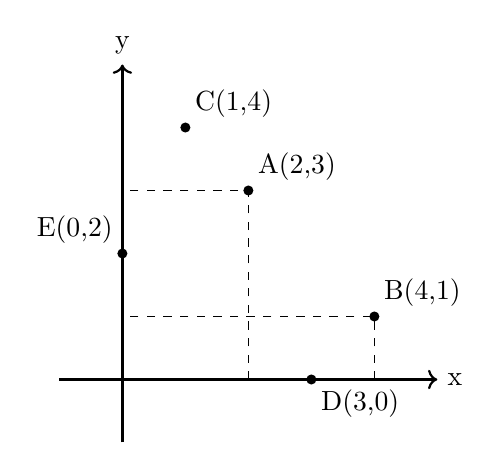
\begin{tikzpicture}[scale=0.8]
    % Eixos
    \draw[->, thick] (-1,0) -- (5,0) node[right] {x};
    \draw[->, thick] (0,-1) -- (0,5) node[above] {y};
    % Pontos
    \filldraw (2,3) circle (2pt) node[above right] {A(2,3)};
    \filldraw (4,1) circle (2pt) node[above right] {B(4,1)};
    \filldraw (1,4) circle (2pt) node[above right] {C(1,4)};
    \filldraw (3,0) circle (2pt) node[below right] {D(3,0)};
    \filldraw (0,2) circle (2pt) node[above left] {E(0,2)};
    % Linhas guia
    \draw[dashed] (2,0) -- (2,3) -- (0,3);
    \draw[dashed] (4,0) -- (4,1) -- (0,1);
\end{tikzpicture}
\end{center}

\section*{2. Representação Gráfica de Funções}

\subsection*{2.1 Conceito Fundamental}
Uma função f associa cada x ∈ D (domínio) a um único y = f(x) ∈ Im (imagem).

\begin{center}
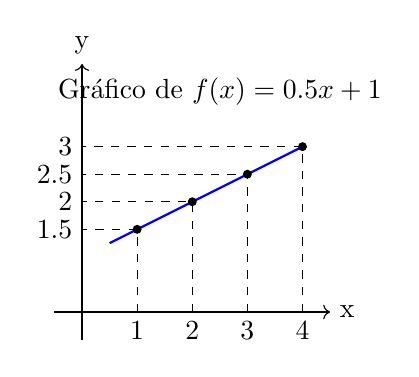
\begin{tikzpicture}[scale=0.7]
    % Plano cartesiano
    \draw[->] (-0.5,0) -- (4.5,0) node[right] {x};
    \draw[->] (0,-0.5) -- (0,4.5) node[above] {y};
    % Função
    \draw[blue, thick, domain=0.5:4] plot (\x, {0.5*\x + 1});
    % Pontos
    \foreach \x/\y in {1/1.5, 2/2, 3/2.5, 4/3} {
        \filldraw (\x,\y) circle (2pt);
        \draw[dashed] (\x,0) node[below] {$\x$} -- (\x,\y) -- (0,\y) node[left] {$\y$};
    }
    % Legenda
    \node at (2.5,4) {Gr\'afico de $f(x) = 0.5x + 1$};
\end{tikzpicture}
\end{center}

\subsection*{2.2 Tipos de Funções}

\subsubsection*{Função Linear}
$f(x) = ax + b$ \\
Gr\'afico: reta com inclinação a

\begin{center}
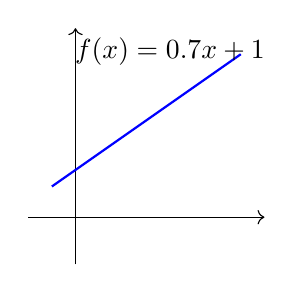
\begin{tikzpicture}[scale=0.6]
    \draw[->] (-1,0) -- (4,0);
    \draw[->] (0,-1) -- (0,4);
    \draw[blue, thick, domain=-0.5:3.5] plot (\x, {0.7*\x + 1});
    \node at (2,3.5) {$f(x) = 0.7x + 1$};
\end{tikzpicture}
\end{center}

\subsubsection*{Função Quadrática}
$f(x) = ax^2 + bx + c$ \\
Gr\'afico: parábola

\begin{center}
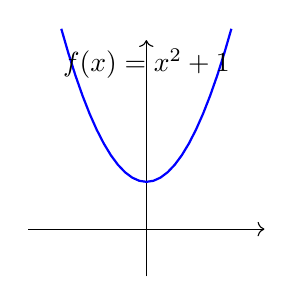
\begin{tikzpicture}[scale=0.6]
    \draw[->] (-2.5,0) -- (2.5,0);
    \draw[->] (0,-1) -- (0,4);
    \draw[blue, thick, domain=-1.8:1.8] plot (\x, {\x*\x + 1});
    \node at (0,3.5) {$f(x) = x^2 + 1$};
\end{tikzpicture}
\end{center}

\section*{3. Exercícios Básicos}

\subsection*{3.1 Identificação de Pontos}
Marque os pontos no plano cartesiano abaixo:

\begin{center}
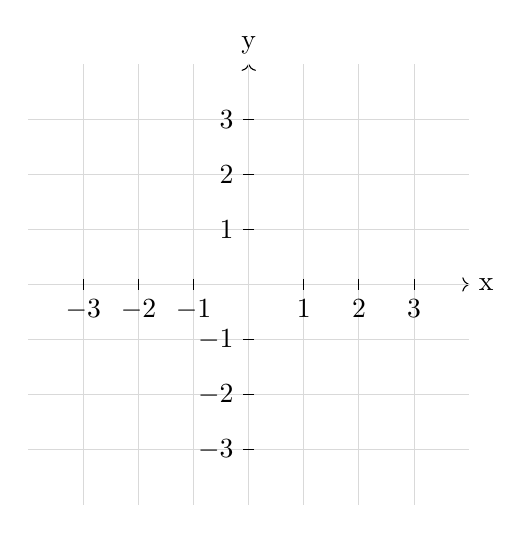
\begin{tikzpicture}[scale=0.7]
    % Eixos
    \draw[->] (-4,0) -- (4,0) node[right] {x};
    \draw[->] (0,-4) -- (0,4) node[above] {y};
    % Grade
    \foreach \x in {-3,-2,...,3} {
        \draw[gray!30] (\x,-4) -- (\x,4);
        \draw[gray!30] (-4,\x) -- (4,\x);
    }
    % Marcas
    \foreach \x in {-3,-2,-1,1,2,3} {
        \draw (\x,0.1) -- (\x,-0.1) node[below] {$\x$};
        \draw (0.1,\x) -- (-0.1,\x) node[left] {$\x$};
    }
\end{tikzpicture}
\end{center}

\begin{enumerate}
    \item A(2,3)
    \item B(-1,2)
    \item C(0,-3)
    \item D(-2,-1)
    \item E(3,0)
\end{enumerate}

\subsection*{3.2 Leitura de Gráficos}
Observe o gráfico e responda:

\begin{center}
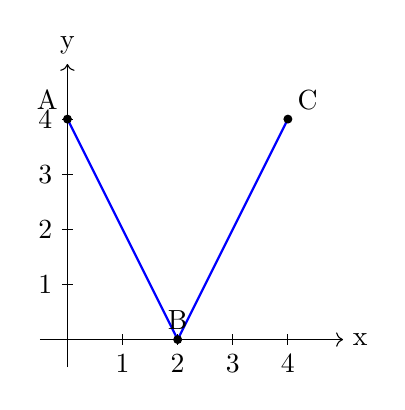
\begin{tikzpicture}[scale=0.7]
    % Eixos
    \draw[->] (-0.5,0) -- (5,0) node[right] {x};
    \draw[->] (0,-0.5) -- (0,5) node[above] {y};
    % Função
    \draw[blue, thick] (0,4) -- (2,0) -- (4,4);
    % Pontos importantes
    \filldraw (0,4) circle (2pt) node[above left] {A};
    \filldraw (2,0) circle (2pt) node[above] {B};
    \filldraw (4,4) circle (2pt) node[above right] {C};
    % Marcas
    \foreach \x in {1,2,3,4} {
        \draw (\x,0.1) -- (\x,-0.1) node[below] {$\x$};
        \draw (0.1,\x) -- (-0.1,\x) node[left] {$\x$};
    }
\end{tikzpicture}
\end{center}

\begin{enumerate}
    \item Quais as coordenadas dos pontos A, B e C?
    \item Qual o valor de y quando $x = 1$?
    \item Para quais valores de x temos $y = 2$?
\end{enumerate}

\section*{4. Exercícios Intermediários}

\subsection*{4.1 Construção de Gráficos}
Esboce os gráficos das seguintes funções no plano abaixo:

\begin{center}
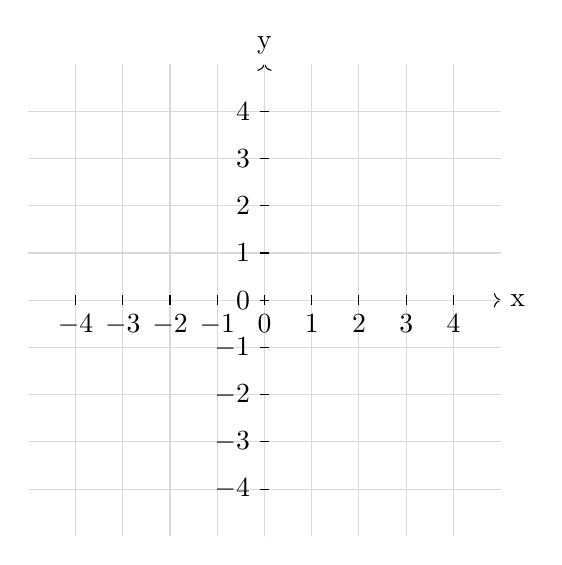
\begin{tikzpicture}[scale=0.6]
    % Eixos
    \draw[->] (-5,0) -- (5,0) node[right] {x};
    \draw[->] (0,-5) -- (0,5) node[above] {y};
    % Grade
    \foreach \x in {-4,-3,...,4} {
        \draw[gray!30] (\x,-5) -- (\x,5);
        \draw[gray!30] (-5,\x) -- (5,\x);
    }
    % Marcas
    \foreach \x in {-4,-3,...,4} {
        \draw (\x,0.1) -- (\x,-0.1) node[below] {$\x$};
        \draw (0.1,\x) -- (-0.1,\x) node[left] {$\x$};
    }
\end{tikzpicture}
\end{center}

\begin{enumerate}
    \item $f(x) = 2x - 1$
    \item $g(x) = -x^2 + 4$
\end{enumerate}

\subsection*{4.2 Análise de Gráficos}
Dado o gráfico da função f:

\begin{center}
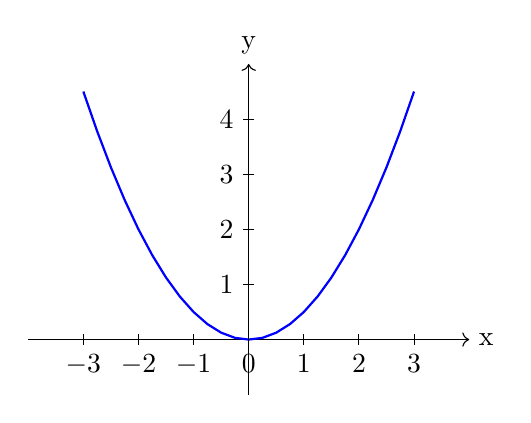
\begin{tikzpicture}[scale=0.7]
    % Eixos
    \draw[->] (-4,0) -- (4,0) node[right] {x};
    \draw[->] (0,-1) -- (0,5) node[above] {y};
    % Função
    \draw[blue, thick, domain=-3:3] plot (\x, {0.5*\x*\x});
    % Marcas
    \foreach \x in {-3,-2,...,3} {
        \draw (\x,0.1) -- (\x,-0.1) node[below] {$\x$};
    }
    \foreach \y in {1,2,3,4} {
        \draw (0.1,\y) -- (-0.1,\y) node[left] {$\y$};
    }
\end{tikzpicture}
\end{center}

\begin{enumerate}
    \item Determine o domínio e a imagem da função
    \item Calcule f(-2), f(0) e f(2)
    \item Para quais valores de x temos $f(x) = 2$?
\end{enumerate}

\section*{5. Exercícios Desafiadores}

\subsection*{5.1 Interseções com os Eixos}
Determine as interseções com os eixos x e y das funções:

\begin{enumerate}
    \item $f(x) = x + 1$
    \item $g(x) = 2x + 1$
    \item $h(x) = \frac{x}{2}$
\end{enumerate}

\subsection*{5.2 Problemas Aplicados}
\begin{enumerate}
    \item Um móvel se desloca em linha reta com velocidade constante. Sua posição em função do tempo é dada por $s(t) = 3t + 5$, onde t está em horas e s em km.
    \begin{enumerate}
        \item Esboce o gráfico da função
        \item Qual a posição inicial do móvel?
        \item Em que instante o móvel estará na posição 20 km?
    \end{enumerate}
    
    \item A área de um quadrado é função do seu lado: $A(l) = l²$. Construa o gráfico dessa função para $l \in [0,5]$ e determine:
    \begin{enumerate}
        \item A área quando $l = 3$
        \item O lado quando $A = 16$
    \end{enumerate}
\end{enumerate}

\end{multicols}

\end{document}
